\documentclass[11pt,a4paper]{article}
\pdftrailerid{adr1d-numerical-validation-2026-07-21-en-v1}

\usepackage[T1]{fontenc}
\usepackage[utf8]{inputenc}
\usepackage[english]{babel}
\usepackage{lmodern}
\usepackage{microtype}
\usepackage[a4paper,margin=2.35cm,headheight=15pt]{geometry}
\usepackage{amsmath,amssymb}
\usepackage{booktabs}
\usepackage{tabularx}
\usepackage{longtable}
\usepackage{array}
\usepackage{graphicx}
\usepackage{caption}
\usepackage{float}
\usepackage{enumitem}
\usepackage{xcolor}
\usepackage{fancyhdr}
\usepackage{hyperref}
\usepackage{xurl}

\definecolor{adrblue}{HTML}{1F5A7A}
\definecolor{adrgreen}{HTML}{2F6B4F}
\definecolor{adrred}{HTML}{9C2F3F}
\definecolor{lightgray}{HTML}{F3F5F6}

\hypersetup{
    colorlinks=true,
    linkcolor=adrblue,
    citecolor=adrgreen,
    urlcolor=adrblue,
    pdftitle={Independent Numerical Validation of ADR1D-ML and ADR1D-NN},
    pdfauthor={Gerardo Tinoco-Guerrero, Francisco J. Domínguez-Mota, J. Alberto Guzmán-Torres}
}

\captionsetup{font=small,labelfont=bf}
\addto\captionsenglish{\renewcommand{\tablename}{Table}}
\setlist[itemize]{leftmargin=*,itemsep=3pt,topsep=5pt}
\setlist[enumerate]{leftmargin=*,itemsep=3pt,topsep=5pt}
\setlength{\parindent}{0pt}
\setlength{\parskip}{5pt}
\setcounter{tocdepth}{2}
\renewcommand{\arraystretch}{1.18}
\newcolumntype{Y}{>{\raggedright\arraybackslash}X}
\newcolumntype{C}{>{\centering\arraybackslash}p{1.7cm}}
\newcommand{\code}[1]{\texttt{#1}}
\newcommand{\pass}{\textcolor{adrgreen}{\textbf{Pass}}}
\newcommand{\mixed}{\textcolor{adrred}{\textbf{Mixed evidence}}}

\pagestyle{fancy}
\fancyhf{}
\lhead{\small ADR1D-ML and ADR1D-NN}
\rhead{\small Numerical validation report}
\cfoot{\thepage}

\begin{document}

\pagenumbering{roman}
\begin{titlepage}
\centering
\vspace*{2.2cm}
{\color{adrblue}\rule{\textwidth}{1.2pt}}\\[1.1cm]
{\Huge\bfseries Independent Numerical Validation of\\[0.25cm]
ADR1D-ML and ADR1D-NN\par}
\vspace{0.65cm}
{\Large Reproducible Technical Report\par}
\vspace{1.1cm}
{\large
Gerardo Tinoco-Guerrero\\[0.15cm]
Francisco J. Domínguez-Mota\\[0.15cm]
J. Alberto Guzmán-Torres\par}
\vspace{0.65cm}
{\normalsize
Universidad Michoacana de San Nicolás de Hidalgo\\
Morelia, Michoacán, Mexico\par}
\vspace{0.25cm}
{\normalsize Contact: \href{mailto:gerardo.tinoco@umich.mx}{gerardo.tinoco@umich.mx}\par}
\vfill
\begin{minipage}{0.88\textwidth}
\small
\textbf{Protocol identifier:} \code{ADR1D-NUMERICAL-VALIDATION} v1.0.0\\
\textbf{Report version:} 1.1, explanatory revision\\
\textbf{Scheduled development period:} May--June 2025\\
\textbf{Last update:} July 2026\\
\textbf{Protocol lock date:} July 21, 2026
\end{minipage}
\vfill
{\normalsize July 21, 2026\par}
\vspace{0.5cm}
{\color{adrblue}\rule{\textwidth}{1.2pt}}
\end{titlepage}
\pagenumbering{arabic}

\begin{abstract}
This report examines two one-dimensional reactive-transport tasks. In the
first, ADR1D-ML estimates effective properties from six noisy sensor histories.
In the second, ADR1D-NN computes concentration divided by inlet concentration
when those properties are already known. The models and their thresholds were
frozen before a challenge set of 120 new scenarios was constructed within the
ADR1D domain. Each inverse scenario had five noise realizations; the neural
field test comprised 299,880 position--time pairs. Samples, metrics,
tolerances, and seeds were specified in advance. As an additional check, 16
scenarios were solved with finite volumes on three meshes and compared with the
analytical solution. Computational cost was measured by component on one CPU
thread.

ADR1D-ML met the prespecified criteria. Median absolute percentage error was
3.95\,\% for effective velocity and 24.94\,\% for effective dispersion. The
classification of whether decay could be distinguished from noise achieved a
balanced accuracy of 0.8357 and an area under the receiver operating
characteristic (ROC) curve of 0.9113; however, 15 of 34 positive declarations
were false positives. ADR1D-NN achieved a global root mean squared error (RMSE)
of 0.02258 on the normalized scale and $R^2=0.98937$. It produced no values
outside $[0,1]$ and exactly satisfied the conditions imposed by its interface
by construction. Favorable average performance coexisted with localized
errors: at the worst point, the reference was zero when the source switched on
at the first interior position, whereas the network predicted 0.74945.

The finite-volume solution reduced its error under refinement in all 16 cases,
and every fine mesh remained within the analytical tolerance. Two cases with
$\mathrm{Pe}=350$ exceeded the medium-to-fine tolerance by 6.9\,\% and
7.4\,\%; the numerical evidence is therefore retained as mixed. The analytical
solution was the fastest field workload, and the timed tasks are not
equivalent, so no universal speed-up is claimed. The models can be integrated
into controlled experiments within ADR1D, but they were validated separately:
the neural field received true parameters rather than those estimated by
ADR1D-ML. This study does not demonstrate chained-workflow performance, field
validation, extrapolation, or fitness for regulatory use.
\end{abstract}

\textbf{Keywords:} contaminant transport; machine learning; neural network;
numerical validation; analytical solution; finite volumes; reproducibility.

\newpage
\tableofcontents
\clearpage

\section{Purpose and Scope}

The transport of a dissolved substance in the subsurface can be studied from
two complementary directions. In the \emph{forward problem}, transport
properties are known and the change in concentration over space and time is
computed. In the \emph{inverse problem}, concentration curves are observed and
the properties that produced them are recovered. In either case, favorable
aggregate performance can conceal local errors: a front may, for example,
arrive too early even when the average field remains close to the reference.

The purpose of this study is to determine, from verifiable evidence, which
claims can be sustained about two models that represent these directions.
ADR1D-ML solves the inverse problem, whereas ADR1D-NN approximates the forward
problem. Both were developed from ADR1D version 1.0.0, a synthetic benchmark
for one-dimensional reactive transport with parameters that remain constant
within each scenario \cite{adr1d}. Their functions are distinct:

\begin{itemize}
    \item \textbf{ADR1D-ML} receives six noisy sensor time histories. From
    these data, it estimates effective velocity, effective dispersion, whether
    decay can be distinguished from the noise level, and, only when that
    distinction is physically resolvable, a decay rate \cite{adr1dml}.
    \item \textbf{ADR1D-NN} receives a position, a time, the effective
    parameters, and the temporal definition of the source. It returns
    concentration divided by inlet concentration, that is, a dimensionless
    field value at that point \cite{adr1dnn}.
\end{itemize}

This difference precludes interpreting their metrics or execution times as a
competition between models: one produces scenario-level parameters and the
other produces pointwise concentration values. The aim is to verify accuracy,
physical consistency, regime sensitivity, reproducibility, and computational
cost separately under defined input contracts. Here, \emph{independent} means
that the protocol was specified before the challenge was examined, the models
were frozen, the new samples were not used for training, and the audit was
performed from persisted files. It does not mean that a different physical
theory was used: the challenge retains the ADR1D equation and parameter ranges.

The study is not intended to replace a site-specific hydrogeological
assessment, demonstrate behavior outside the training ranges, or attribute to
Water Quality Portal observations hydraulic variables that those records do
not contain. The conclusions are restricted to the synthetic problem defined
in this document.

The validation questions were as follows:

\begin{enumerate}
    \item Can the published canonical results be reproduced without modifying
    the models or their protocols?
    \item Do both models maintain acceptable performance on new scenarios that
    were generated before inference and do not collide with the canonical set?
    \item Where are errors concentrated, and how do they differ across
    physical regimes, interior samples, and boundary profiles?
    \item Does the analytical reference agree with an independent traditional
    discretization as space and time are refined?
    \item What is the observed cost of each component under an explicit and
    reproducible measurement policy?
\end{enumerate}

\subsection{Reading Guide and Terminology}

The report deliberately separates the physical reference, input data, model
queries, and subsequent diagnostics. Table~\ref{tab:vocabulary} summarizes
terms used throughout the text.

\begin{table}[htbp]
\centering
\caption{Operational terminology used in the validation.}
\label{tab:vocabulary}
\small
\begin{tabularx}{\textwidth}{@{}>{\raggedright\arraybackslash}p{3.6cm}Y@{}}
\toprule
Term & Meaning in this report \\
\midrule
Base scenario & A complete combination of physical and source parameters. It
is the independent unit of analysis. \\
Noise realization & A distinct synthetic observation of the same scenario;
only the sensor noise changes. \\
Space--time point & An $(x,t)$ pair within a scenario. Points on the same mesh
are correlated and are not counted as independent experiments. \\
Analytical reference & Value computed from the closed-form ADR1D solution
using the true scenario parameters. \\
Traditional reference & Solution obtained with the independent finite-volume
method described in Section~\ref{sec:numerical-method}. \\
Frozen model & Model file identified and locked before the challenge, with no
subsequent retraining or adjustment. \\
Active region & Points for which the normalized reference concentration is
greater than $10^{-4}$. \\
Prespecified criterion & Tolerance recorded before inference. A failure is
retained and does not trigger a change in the threshold or model. \\
\bottomrule
\end{tabularx}
\end{table}

\section{Physical Problem and Evaluated Artifacts}

\subsection{Transport Equation}

ADR1D represents transport in a homogeneous medium through

\begin{equation}
R\frac{\partial C}{\partial t}
=D\frac{\partial^2 C}{\partial x^2}
-v\frac{\partial C}{\partial x}
-\lambda R C,
\label{eq:adr}
\end{equation}

where $C$ is dissolved concentration, $D$ is longitudinal dispersion, $v$ is
advective velocity, $R$ is the retardation factor, and $\lambda$ is the
first-order decay rate. Coordinate $x$ increases along the mean flow direction,
and $t$ is the time elapsed since the beginning of the experiment.
Table~\ref{tab:variables} lists the units and interpretation.

\begin{table}[htbp]
\centering
\caption{Variables and parameters of the transport equation.}
\label{tab:variables}
\small
\begin{tabularx}{\textwidth}{@{}p{1.6cm}p{2.4cm}Y@{}}
\toprule
Symbol & Unit & Interpretation \\
\midrule
$C(x,t)$ & mg L$^{-1}$ & Dissolved concentration at position $x$ and time $t$. \\
$v$ & m s$^{-1}$ & Advective velocity before retardation is applied. It
translates the center of the pulse. \\
$D$ & m$^2$ s$^{-1}$ & Longitudinal dispersion coefficient. It controls
broadening of the front and tail. \\
$R$ & Dimensionless & Retardation factor. A value greater than one reduces the
effective solute velocity and dispersion relative to the reference flow. \\
$\lambda$ & s$^{-1}$ & First-order loss rate. In the absence of transport,
concentration decreases as $\exp(-\lambda t)$. \\
$C_0$ & mg L$^{-1}$ & Concentration prescribed at the inlet while the source
remains active. \\
$t_0,\tau$ & s & Source activation time and inlet-pulse duration. \\
\bottomrule
\end{tabularx}
\end{table}

The three terms on the right-hand side of Equation~\eqref{eq:adr} have distinct
roles. The second-derivative term smooths gradients through dispersion, the
first-derivative term transports the profile, and $-\lambda RC$ reduces the
concentration. Dividing by $R$ defines $D_{\mathrm{eff}}=D/R$ and
$v_{\mathrm{eff}}=v/R$:

\begin{equation}
\frac{\partial C}{\partial t}
=D_{\mathrm{eff}}\frac{\partial^2 C}{\partial x^2}
-v_{\mathrm{eff}}\frac{\partial C}{\partial x}
-\lambda C.
\label{eq:effective}
\end{equation}

This form shows which parameters the models receive: ADR1D-ML attempts to
recover $v_{\mathrm{eff}}$ and $D_{\mathrm{eff}}$, whereas ADR1D-NN receives
them as known inputs. Decay retains the rate $\lambda$ because $R$ appears in
both the temporal and reaction terms of Equation~\eqref{eq:adr}.

Scenarios with different source concentrations are compared using

\begin{equation}
c(x,t)=\frac{C(x,t)}{C_0}.
\label{eq:normalized-concentration}
\end{equation}

Variable $c$ is dimensionless. In the benchmark, its reference value is zero
before arrival and one at the inlet during the pulse. An RMSE of 0.02 in this
field therefore corresponds to a root mean squared error of two percentage
points relative to $C_0$; it is not 0.02 mg L$^{-1}$ unless $C_0=1$
mg L$^{-1}$.

The initial condition is $C(x,0)=0$. At $x=0$, a rectangular pulse is prescribed,

\begin{equation}
C(0,t)=
\begin{cases}
C_0, & t_0\leq t<t_0+\tau,\\
0, & \text{otherwise},
\end{cases}
\end{equation}

and the analytical solution assumes decay in the far field. ADR1D evaluates a
reactive extension of the Ogata--Banks-type response
\cite{ogata1961,chen2011}. If $u=(v^2+4\lambda R D)^{1/2}$, the unit-step
response is

\begin{align}
S(x,t)={}&\frac{1}{2}\exp\!\left(\frac{(v-u)x}{2D}\right)
\operatorname{erfc}\!\left(\frac{Rx-ut}{2\sqrt{DRt}}\right)\notag\\
&+\frac{1}{2}\exp\!\left(\frac{(v+u)x}{2D}\right)
\operatorname{erfc}\!\left(\frac{Rx+ut}{2\sqrt{DRt}}\right),
\end{align}

for $t>0$, and the pulse is obtained as
$C(x,t)=C_0[S(x,t-t_0)-S(x,t-t_0-\tau)]$. This expression avoids associating
reference labels with the error of a particular numerical mesh. Function
$\operatorname{erfc}$ is the complementary error function. When the elapsed
time supplied to $S$ is less than or equal to zero, the response is defined as
zero. Subtracting two step responses has a direct interpretation: the first
switches the source on at $t_0$, and the second removes, after $\tau$, the
contribution of a source that would otherwise have remained active.

The closed-form solution is defined on a semi-infinite domain. The benchmark
retains the first $L=1000$ m and the first 24 h. The finite-volume reference,
which requires an outlet boundary, extends the domain to 1200 m and avoids
comparisons near that outlet; this distinction is detailed in
Section~\ref{sec:numerical-method}.

The following quantities are used to interpret the design extremes:

\begin{equation}
\mathrm{Pe}=\frac{v_{\mathrm{eff}}L}{D_{\mathrm{eff}}},
\qquad
\mathrm{Da}=\frac{\lambda L}{v_{\mathrm{eff}}},
\end{equation}

with $L=1000$ m. The four regimes combine active or inactive retardation with
active or zero decay: conservative, decay only, retardation only, and
retardation with decay. The Peclet number compares advection and dispersion:
large values correspond to narrower fronts dominated by advective transport,
whereas small values correspond to more diffuse profiles. The Damköhler number
compares the decay scale with the advective travel time: $\mathrm{Da}=0$
indicates no decay, and larger values imply more visible attenuation over the
travel length $L$.

\begin{table}[htbp]
\centering
\caption{Physical regimes in the design. ``Active'' means that the parameter is
sampled over its interval; ``inactive'' fixes $R=1$ or $\lambda=0$.}
\label{tab:regimes}
\small
\begin{tabularx}{\textwidth}{@{}YccY@{}}
\toprule
Regime & Retardation & Decay & Physical interpretation \\
\midrule
Conservative & Inactive & Inactive & Transport without reactive loss or an
additional reduction due to retardation. \\
Decay only & Inactive & Active & First-order attenuation during transport. \\
Retardation only & Active & Inactive & Lower effective velocity and dispersion,
without reaction-driven mass loss. \\
Retardation and decay & Active & Active & Simultaneous retardation and
attenuation. \\
\bottomrule
\end{tabularx}
\end{table}

\subsection{Frozen Models}

The artifacts were treated as closed boxes with public interfaces. The
serialized ADR1D-ML bundle and the ADR1D-NN weights and transformations
checkpoint were identified in their manifests and lock records before the
challenge. Their integrity was verified before and after every operation that
loaded a model. Retraining, further hyperparameter selection, changes to the
classification threshold, and post hoc correction of challenge results were
not permitted.

\subsubsection{ADR1D-ML Inverse Workflow}

Each realization supplied to ADR1D-ML contains 294 observations: 49 times at
each of six sensors. The interface does not provide these 294 concentrations
directly to a single estimator. It first summarizes each sensor through eleven
descriptors: detected fraction, peak-to-$C_0$ ratio, peak time, first and last
detection, normalized area, centroid, temporal spread, and cumulative times at
10, 50, and 90\,\% of the area. The 66 sensor descriptors, together with
$C_0$, $t_0$, and $\tau$, form 69 features per realization.

Velocity and dispersion are estimated by two independent ensembles of 300
extremely randomized trees. Both predict the base-ten logarithm of the positive
parameter and use median imputation when a temporal descriptor cannot be
computed, for example, because a sensor records no signal above the detection
limit. The logarithmic transformation accommodates multiplicative errors and
prevents negative physical predictions after conversion back to the original
units.

Decay classification adds 17 descriptors that compare sensors at different
distances. These include slopes of peaks, areas, centroids, and times; the
quality of those fits; and physical approximations of velocity, dispersion,
and attenuation. A logistic regression with 86 inputs estimates the
probability that decay is resolvable. The classification truth was defined
before training as

\begin{equation}
a_{\lambda}=1-\exp(-\mathrm{Da}), \qquad
y_{\mathrm{res}}=\mathbb{I}\!\left(a_{\lambda}\geq0.03\right),
\label{eq:resolvability}
\end{equation}

so that the physical threshold is
$\mathrm{Da}\geq-\ln(0.97)=0.0304592$. In words, decay is labeled resolvable
when its ideal attenuation over one travel time is at least as large as the
3\,\% relative noise. This label expresses resolvability within the benchmark;
it does not signify the chemical presence or absence of a reaction. A positive
rate below the threshold is considered unresolvable with these sensors and
this noise level.

The probability is converted to the positive class when it is greater than or
equal to 0.19, a threshold selected during development and frozen before the
test. Only for scenarios whose truth satisfies Equation~\eqref{eq:resolvability}
does a fourth 300-tree model estimate $\log_{10}\lambda$ from twelve selected
descriptors. This separation avoids reporting a numerical estimate of
$\lambda$ when the expected effect falls below the defined resolution.

The five noise realizations produce five predictions per scenario. If
$\widehat z_r>0$ denotes a positive prediction from replicate $r$, the summary
is their geometric mean:

\begin{equation}
\widehat z_{\mathrm{esc}}
=\exp\!\left(\frac{1}{5}\sum_{r=1}^{5}\ln\widehat z_r\right).
\end{equation}

Probabilities are averaged arithmetically, and the 0.19 threshold is applied
once to that average. Each scenario thus contributes one observation to the
primary metrics, while variation among replicates is retained as a diagnostic
of noise sensitivity.

\subsubsection{ADR1D-NN Forward Workflow}

ADR1D-NN is a coordinate- and parameter-conditioned neural surrogate. Its
interface receives nine columns: $x$, $t$, $L$, final time,
$v_{\mathrm{eff}}$, $D_{\mathrm{eff}}$, $\lambda$, $t_0$, and $\tau$. From
these columns it constructs seven network inputs: normalized position and time,
logarithms of effective velocity and dispersion, a
$\log(1+\lambda/10^{-6})$ transformation, normalized source start time, and
normalized duration. The means and standard deviations used to standardize
these inputs are stored in the checkpoint.

The network is a multilayer perceptron with three hidden layers of 128 neurons,
SiLU activation, a sigmoid output, and 34,177 trainable parameters. The
checkpoint corresponds to epoch 57, selected with the validation set during
development. The sigmoid output keeps neural predictions between zero and one.
Because Equation~\eqref{eq:effective} is linear in concentration, $C_0$ is not
a network input: dimensional units are recovered as
$\widehat C=C_0\widehat c$.

The interface replaces the network output with exact values on two sets:
$c(x,0)=0$ for $x>0$, and the rectangular pulse at $x=0$. The order of
application also resolves the corner $(0,0)$ according to the inlet condition.
At all remaining interior points, including times near source activation and
deactivation, the prediction comes from the network. Consequently, satisfying
these two conditions verifies the implemented contract, but does not by itself
demonstrate local conservation or exact satisfaction of the differential
equation.

\section{Validation Design}

\subsection{Prior Lock and Separation of Evidence}

The protocol, its inputs, and the tolerances were locked before any cases were
generated or new inference was executed. The initial record verified 18 frozen
inputs and left the counters for new scenarios, challenge inferences, and
traditional solutions at zero. Three levels of evidence were then followed:

\begin{enumerate}
    \item \textbf{Canonical reproduction.} The previously published tests for
    45 scenarios were repeated without using the challenge set.
    \item \textbf{Independent challenge.} A total of 120 scenarios were
    generated, verified, and locked before one persisted inference per model.
    \item \textbf{Traditional numerical reference.} Sixteen scenarios were
    selected using only true parameters and solved at three mesh levels.
\end{enumerate}

The operational sequence was to (1) register the protocol, models, code, and
canonical data; (2) generate the new set without loading models; (3) reconstruct
it with a separate validator; (4) lock the set and its records; (5) prepare
input tables without inference; (6) execute one persisted query per model; and
(7) recalculate metrics from the CSV files with an auditor that neither imports
the evaluator nor deserializes the models. The traditional reference was run
afterward on scenarios selected solely from true parameters.

This sequence avoids two forms of optimism. First, it prevents case selection
after learning where the models perform best. Second, it prevents changing a
threshold or transformation to improve the result retrospectively. New metrics
were not used to modify the models. A failed criterion had to be retained and
discussed in the same detail as a favorable result.

\subsection{Challenge Set}

The design included 30 scenarios per regime: 24 interior points obtained by
Latin hypercube sampling \cite{mckay1979} and six boundary profiles.
Table~\ref{tab:ranges} summarizes the ranges. Positive variables spanning
several orders of magnitude were sampled on a logarithmic scale; the others
were sampled linearly. In Latin hypercube sampling, each transformed interval
is divided into 24 strata, and each stratum is used once per dimension. This
improves interval coverage with fewer points than a Cartesian grid, but does
not turn the scenarios into a sample of naturally occurring aquifer
frequencies.

\begin{table}[htbp]
\centering
\caption{Ranges of the locked challenge set.}
\label{tab:ranges}
\begin{tabular}{@{}lll@{}}
\toprule
Variable & Range & Design transformation \\
\midrule
Velocity $v$ & 0.05--0.35 m s$^{-1}$ & Linear \\
Dispersion $D$ & 1--20 m$^2$ s$^{-1}$ & $\log_{10}$ \\
Source concentration $C_0$ & 0.2--5 mg L$^{-1}$ & $\log_{10}$ \\
Source start $t_0$ & 0--3600 s & Linear \\
Duration $\tau$ & 1800--10800 s & Linear \\
Active retardation $R$ & 1.1--3.0 & Linear \\
Active decay $\lambda$ & $10^{-7}$--$2\times10^{-5}$ s$^{-1}$ & $\log_{10}$ \\
\bottomrule
\end{tabular}
\end{table}

The six boundary profiles per regime are not random observations. The first
four combine the minimum and maximum velocity and dispersion values while
holding all other transformed coordinates at their midpoints. The remaining
two combine opposing extremes of concentration, start time, duration,
retardation, and decay. Their purpose is to expose the model to documented
corners of the domain that open interior sampling does not reach exactly. When
a process is inactive in a regime, $R=1$ or $\lambda=0$ is fixed.

The neural network receives effective parameters. Because of division by $R$,
the covered effective range is approximately 0.0167--0.35 m s$^{-1}$ for
velocity and 0.333--20 m$^2$ s$^{-1}$ for dispersion. Every challenge case
remains within the strict ADR1D-ML and ADR1D-NN input contracts; the boundary
profiles test permitted extremes, not extrapolation.

Each scenario field contains 51 positions between 0 and 1000 m and 49 times
between 0 and 86400 s, for a total of 299,880 values. ADR1D-ML used six sensors
at 100, 250, 400, 600, 800, and 1000 m. Each scenario received five independent
realizations of 3\,\% relative Gaussian noise, an absolute floor of
0.002 mg L$^{-1}$, a detection limit of 0.01 mg L$^{-1}$, and substitution of
0.005 mg L$^{-1}$ below that limit. This produced 600 realizations and 176,400
observations.

For each observation with truth $C_{\mathrm{ref}}$, the following model was
used:

\begin{align}
\sigma(C_{\mathrm{ref}})&=\max\!\left(0.002\ \text{mg L}^{-1},
0.03C_{\mathrm{ref}}\right),\\
C_{\mathrm{uncensored}}&=\max\!\left(0,
C_{\mathrm{ref}}+\sigma Z\right),\qquad Z\sim\mathcal N(0,1).
\label{eq:sensor-noise}
\end{align}

If $C_{\mathrm{uncensored}}<0.01$ mg L$^{-1}$, the value supplied to the
feature workflow was 0.005 mg L$^{-1}$ and was marked as not detected. During
extraction, that mark preserves the frequency of nondetections but assigns zero
to the integrated signal. This convention separates the value used to
represent a report below the detection limit from the value used to compute
area, centroid, and cumulative times.

The parameter seed was 2026072105, the noise seed was 2026072106, and the
bootstrap seed was 2026072107. The validator reconstructed the scenarios,
fields, true concentrations, and every noise sequence without loading the
models. The maximum absolute difference from the reconstruction was
approximately $5.0\times10^{-12}$ mg L$^{-1}$. There were no duplicate
identifiers or parameters relative to the 300 canonical scenarios; the minimum
normalized distance was 0.1170. A second temporary generation produced files
that were identical byte for byte. The distance was computed after mapping
each parameter to its normalized linear or logarithmic coordinate. Thus,
0.1170 indicates separation in design space; it is neither a physical distance
in meters nor a measure of similarity between complete fields.

\subsection{Metrics and Statistical Analysis}

\subsubsection{Regression and Field Errors}

Let $y_i$ be a reference, $\widehat y_i$ its prediction, and
$e_i=\widehat y_i-y_i$. The basic metrics were computed as

\begin{align}
\mathrm{MAE}&=\frac{1}{N}\sum_{i=1}^{N}|e_i|,\\
\mathrm{RMSE}&=\sqrt{\frac{1}{N}\sum_{i=1}^{N}e_i^2},\\
R^2&=1-\frac{\sum_{i=1}^{N}e_i^2}
{\sum_{i=1}^{N}(y_i-\overline y)^2}.
\label{eq:regression-metrics}
\end{align}

Mean absolute error (MAE) expresses the average magnitude of error without
regard to sign. Root mean squared error (RMSE) gives greater weight to large
errors because it squares the residuals. Coefficient $R^2$ compares model error
with the error obtained by always predicting the mean reference value: one
indicates perfect agreement; zero indicates no improvement over that mean; and
a negative value indicates worse performance. A high $R^2$ does not guarantee
a small maximum error or correct front arrival.

For positive parameters spanning several orders of magnitude, the same
equations were applied to $\log_{10}y_i$ and $\log_{10}\widehat y_i$. Absolute
percentage error (APE) was also computed as

\begin{equation}
\mathrm{APE}_i=100\frac{|\widehat y_i-y_i|}{y_i}.
\label{eq:ape}
\end{equation}

Median APE describes a typical scenario, and the 90th percentile indicates the
value below which 90\,\% of scenarios fall. A 90th percentile of 65\,\%, for
example, does not mean that every error is 65\,\%; it means that approximately
one tenth are larger. ADR1D-ML uses one aggregate prediction for each of the
120 scenarios. The conditional evaluation of $\lambda$ uses only the 23
scenarios whose truth is resolvable.

ADR1D-NN was summarized in two ways. \emph{Pooled} metrics use all 299,880
points to describe the complete field. \emph{Per-scenario} metrics are first
computed on each 2499-point mesh and then summarize the distribution of 120
RMSE values. This second view prevents a scenario with a simple or nearly zero
field from determining the conclusion by itself.

\subsubsection{Resolvability Classification}

The confusion matrix distinguishes true positives (TP), true negatives (TN),
false positives (FP), and false negatives (FN). The following metrics were
used:

\begin{align}
\operatorname{Sens}&=\frac{\mathrm{TP}}{\mathrm{TP}+\mathrm{FN}}, &
\operatorname{Spec}&=\frac{\mathrm{TN}}{\mathrm{TN}+\mathrm{FP}},\\
\operatorname{BA}&=\frac{1}{2}
(\operatorname{Sens}+\operatorname{Spec}), &
\operatorname{Prec}&=\frac{\mathrm{TP}}{\mathrm{TP}+\mathrm{FP}},\\
F_1&=2\frac{\operatorname{Prec}\,\operatorname{Sens}}
{\operatorname{Prec}+\operatorname{Sens}}.
\label{eq:classification-metrics}
\end{align}

Sensitivity answers how many resolvable cases were recovered; precision
answers how many positive declarations were correct. Balanced accuracy
averages sensitivity and specificity so that the minority class is not hidden.
The area under the ROC curve evaluates probability ranking across all
thresholds, whereas the confusion matrix and $F_1$ depend on the frozen 0.19
threshold. Log loss penalizes confident probabilities assigned to the wrong
class. These metrics are not interchangeable: a classifier may rank cases well
while producing too many false positives at a particular threshold.

\subsubsection{Physical Diagnostics of the Neural Field}

The active region was defined by $c_{\mathrm{ref}}>10^{-4}$. MAE and RMSE were
reported for both the entire field and this region because broad areas with a
zero or nearly zero reference can artificially lower the global average. The
initial condition, inlet boundary, and fractions of predictions below zero or
above one were also verified.

For each scenario, the spatial integral was first computed as

\begin{equation}
Q(t)=\int_0^L c(x,t)\,dx,
\end{equation}

and then $\mathcal M=\int_0^TQ(t)\,dt$. The diagnostic termed \emph{relative
integrated-mass error} is
$|\widehat{\mathcal M}-\mathcal M|/\mathcal M$. Because $c$ is normalized and
the model does not include cross-sectional area, bulk density, or porosity,
this quantity is a comparative field integral rather than the total
dimensional mass of contaminant in an aquifer.

At each interior position where the reference reaches $10^{-4}$, arrival time
was defined as the first tabulated time above that threshold. The absolute
error between the first reference and predicted arrivals was computed and
summarized per scenario by the spatial median. If the prediction never crossed
the threshold, the final time plus one time step was assigned as a penalty.
Because the field is stored every 1800 s, this diagnostic is quantized in
1800 s intervals.

Finally, the following residual was approximated at interior nodes:

\begin{equation}
r=\frac{\partial \widehat c}{\partial t}
-D_{\mathrm{eff}}\frac{\partial^2\widehat c}{\partial x^2}
+v_{\mathrm{eff}}\frac{\partial\widehat c}{\partial x}
+\lambda\widehat c
\label{eq:pde-residual}
\end{equation}

using centered differences, and its RMSE was reported. This residual depends
on the diagnostic mesh, amplifies abrupt changes, and is not written in
conservative form; it was therefore recorded without an acceptance threshold.

\subsubsection{Independent Unit and Intervals}

The resampling unit was always the base scenario. The 95\,\% intervals were
computed from 5000 replicates of grouped percentile bootstrap resampling
\cite{efron1993}. In each replicate, scenario identifiers were sampled with
replacement, and their five noise realizations or 2499 points were kept
together. Treating every point as an independent observation would have
produced artificially narrow intervals because neighboring values belong to
the same solution and are correlated.

The minimum criteria were specified before the challenge was examined. They
were chosen as sufficiency tolerances for deciding whether the models could
continue to be used in ADR1D experiments, not as regulatory limits or
guarantees for a real case. The intervals describe variation among scenarios
in the design; they are not predictive intervals for an individual scenario.

\subsection{Traditional Numerical Reference}
\label{sec:numerical-method}

The traditional reference was implemented separately from the analytical
generation and ADR1D-NN. Its purpose was not to compete with the network in
execution time, but to answer two questions: whether the closed-form solution
is consistent with a conservative discretization and whether error decreases
as space and time are refined.

Equation~\eqref{eq:effective} can be written as

\begin{equation}
\frac{\partial c}{\partial t}+\frac{\partial J}{\partial x}
=-\lambda c, \qquad
J=v_{\mathrm{eff}}c-D_{\mathrm{eff}}\frac{\partial c}{\partial x}.
\label{eq:conservative-form}
\end{equation}

The domain was divided into volumes of uniform width $\Delta x$, and an average
concentration was stored at the center of each cell. At a face between cells
$i$ and $i+1$, the Scharfetter--Gummel flux was \cite{scharfetter1969}

\begin{equation}
J_{i+1/2}=\frac{D_{\mathrm{eff}}}{\Delta x}
\left[B(-P_h)c_i-B(P_h)c_{i+1}\right],\qquad
P_h=\frac{v_{\mathrm{eff}}\Delta x}{D_{\mathrm{eff}}},
\label{eq:sg-flux}
\end{equation}

where $B(z)=z/(\exp z-1)$ and $B(0)=1$. This fitting reproduces centered
diffusion when $P_h$ is small and avoids the negative oscillations that a
conventional centered approximation can introduce when advection dominates.
The identity $B(-P_h)-B(P_h)=P_h$ ensures that a constant state carries the
correct advective flux.

After the fluxes were assembled, the semidiscrete system took the form
$d\mathbf c/dt=A\mathbf c+\mathbf b c_{\mathrm{in}}(t)$. Each step was solved
with backward Euler:

\begin{equation}
(I-\Delta t A)\mathbf c^{n+1}
=\mathbf c^n+\Delta t\,\mathbf b\,
c_{\mathrm{in}}(t_{n+1/2}).
\label{eq:backward-euler}
\end{equation}

The method is implicit and does not require the stability restriction of an
explicit Euler scheme; its accuracy nevertheless depends on $\Delta t$.
Factorizations were reused whenever the same time step recurred. Times $t_0$
and $t_0+\tau$ were inserted exactly into the time grid so that no step crossed
a source change without representing it.

The computational domain was extended to 1200 m. At the inlet, the Dirichlet
pulse was imposed over a half-cell distance. At the outlet, the diffusive flux
was set to zero and the advective flux $v_{\mathrm{eff}}c$ was allowed. The
comparison was restricted to $0\leq x\leq900$ m to preserve at least 300 m
between reported points and this artificial boundary.

Four scenarios were selected per regime: minimum Peclet, maximum Peclet,
maximum Damköhler or greatest advective travel time when $\lambda=0$, and the
medoid of normalized parameter space. The medoid is the existing scenario with
the smallest total distance to the other points in its regime; unlike a
centroid, it always corresponds to an actual case in the set. Selection did not
consult model or solver errors. The three discretizations were

\begin{center}
\begin{tabular}{@{}lcc@{}}
\toprule
Level & $\Delta x$ & Maximum $\Delta t$ \\
\midrule
Coarse & 10 m & 225 s \\
Medium & 5 m & 112.5 s \\
Fine & 2.5 m & 56.25 s \\
\bottomrule
\end{tabular}
\end{center}

The three meshes are nested. To compare levels, the averages of two adjacent
fine cells were restricted to one cell at the next level; displaced centers
were not compared through arbitrary interpolation. The analytical solution was
evaluated at cell centers and at the 49 reporting times. The empirical order
between successive errors was computed as

\begin{equation}
p=\frac{\log(E_h/E_{h/2})}{\log 2}.
\label{eq:observed-order}
\end{equation}

Because $\Delta x$ and the maximum time step were reduced simultaneously, $p$
describes the joint space--time campaign rather than the isolated asymptotic
order of one discretization.

Balance was checked at every step using the change in the discrete integral,
the outlet flux, inlet flux, and reactive loss:

\begin{equation}
r_{\mathrm{bal}}=
\frac{M^{n+1}-M^n}{\Delta t}
+J_{\mathrm{out}}-J_{\mathrm{in}}+\lambda M^{n+1},
\qquad M^n=\Delta x\sum_i c_i^n.
\label{eq:mass-balance}
\end{equation}

Acceptance required, in each of the 16 cases, a fine-mesh RMSE relative to the
analytical solution no greater than 0.03, an RMSE between the restricted medium
and fine meshes no greater than 0.01, and a minimum concentration no lower than
$-10^{-10}$. Discrete balance, maximum error, arrival time, and observed order
were retained as diagnostics. The first criterion measures agreement with a
reference external to the mesh; the second asks whether two successive
resolutions are already sufficiently close under the adopted tolerance.

\subsection{Computational Cost}

The benchmark was run on a CPU with one computational thread. Each workload
had two warm-ups and seven repetitions measured with
\code{time.perf\_counter\_ns}; median, interquartile range, minimum, and maximum
were reported. Data were loaded into memory before the computational kernels
were timed, so CSV reading and output serialization were excluded.

Separation by component prevents assigning the entire cost to the model.
Loading includes verifying and deserializing the artifact; feature construction
transforms data already resident in memory; inference calls the frozen
estimator; and the end-to-end path combines these three steps while continuing
to exclude file input and output. For the traditional reference, analytical
evaluation, finite-volume integration, and the workflow that prepares the 16
cases and executes both calculations were timed separately.

The two warm-ups initialize deferred imports, caches, and internal paths before
times are summarized. All seven measurements are retained in the JSON so that
the median does not conceal their dispersion. The interquartile range is the
difference between the 75th and 25th percentiles and describes the central half
of the repetitions.

To avoid turning timing into a second query of the challenge set, model times
were measured only on the published canonical partition: 45 scenarios for
ADR1D-ML and 112,455 points for ADR1D-NN. The analytical evaluation and
traditional solver used the 16 selected cases on the fine mesh, with 376,320
retained values. Every repetition produced the same output. A separate probe
with \code{tracemalloc} described allocations visible from Python; it is not
interpreted as total resident memory because it may omit allocations made by
native libraries.

\section{Results}

\subsection{Reproduction and Integrity}

ADR1D-ML reproduced five prediction arrays and four metric checks over its 45
canonical scenarios. ADR1D-NN reproduced 112,455 predictions, 60 scalar
metrics, 45 per-scenario rows, four diagnostic selections, and 4,455 exact
physical constraints. In both cases, the reconstructed report was identical
to the published report byte for byte.

Binary identity is a more demanding test than observing similar figures: it
confirms that, with the same inputs and environment, record order, serialized
precision, and the full report content were preserved. This test establishes
reproducibility of the canonical evaluation; it does not replace the new test
because those 45 scenarios had already been part of the development history.

Challenge inference was executed once per model after locking. No subsequent
adjustment was made. An audit that neither imported the evaluation modules nor
loaded models recalculated the evidence from the CSV files: it completed 2664
checks, compared 2423 values, and found a maximum absolute difference of
$8.92\times10^{-13}$, attributable to serialization precision. The protected
models, protocols, inputs, and results remained unchanged.

The 2664 checks included counts, identifiers, global metrics, per-scenario
results, bootstrap intervals, physical constraints, and integrity checks. The
maximum difference is approximately eleven orders of magnitude smaller than
the model RMSE and therefore reflects file rounding rather than a material
discrepancy between evaluator and auditor.

\subsection{Parameter Estimation with ADR1D-ML}

Figure~\ref{fig:ml} shows scenario-level aggregation. Velocity was recovered
with less relative dispersion than $D_{\mathrm{eff}}$ and $\lambda$. Across
the 120 scenarios, median absolute percentage error for velocity was
3.95\,\%, its 90th percentile was 10.87\,\%, and logarithmic $R^2$ was 0.9892.
The corresponding values for dispersion were 24.94\,\%, 65.81\,\%, and
0.8494.

In distributional terms, half of the velocity estimates deviated by less than
3.95\,\%, and nine out of ten deviated by less than 10.87\,\%. For dispersion,
half remained below 24.94\,\%, but approximately one tenth exceeded 65.81\,\%.
Meeting the dispersion tolerance should not be read as uniform accuracy: the
protocol allowed a larger error for a property that is more difficult to
identify from the broadening of censored curves.

\begin{figure}[!t]
\centering
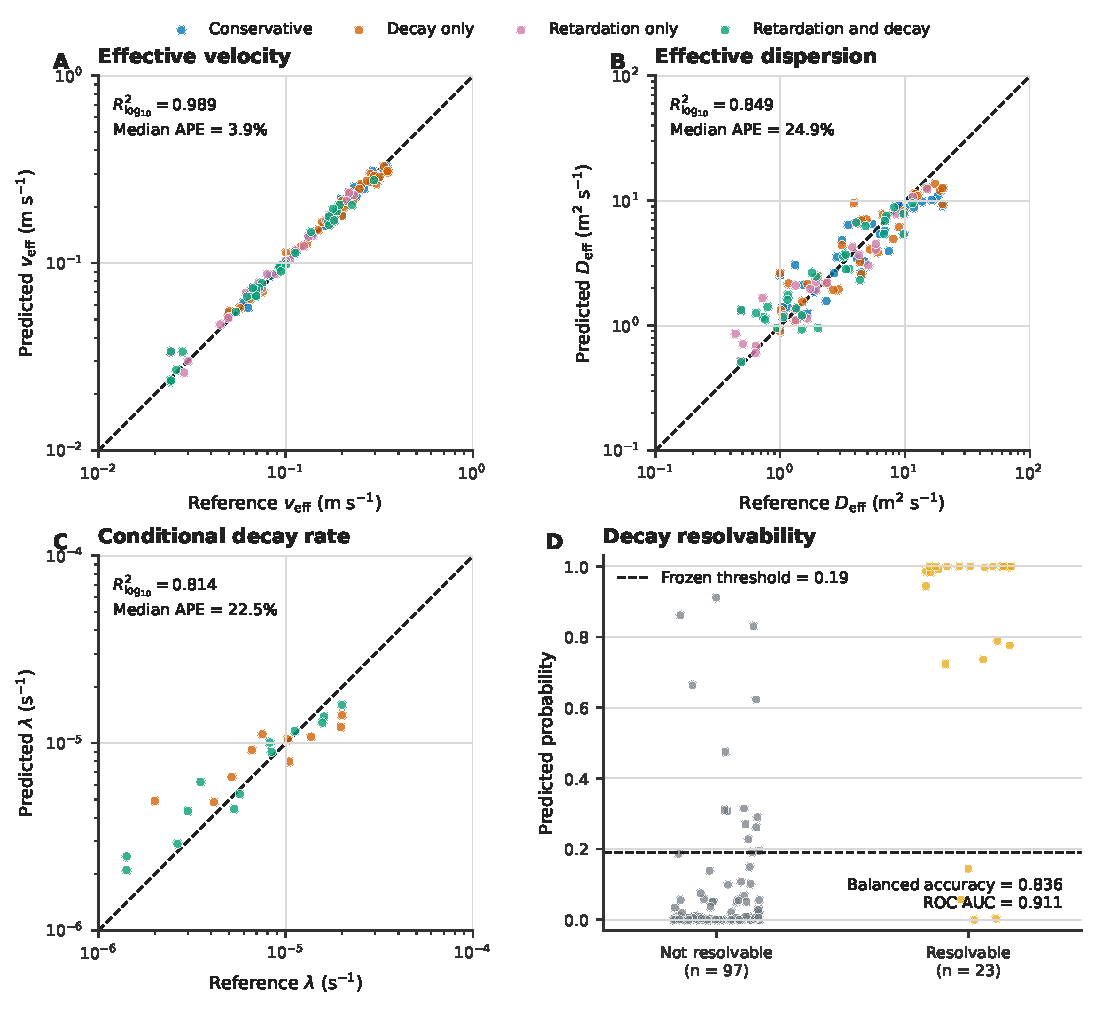
\includegraphics[width=0.91\textwidth]{figures/figure_01_parameter_model_validation.pdf}
\caption{Validation of ADR1D-ML on 120 new scenarios. (A--C) Agreement between
the reference and aggregate prediction; the dashed line indicates identity.
(D) Probability of decay resolvability and the frozen threshold. Each point
represents one base scenario, not an individual noise realization.}
\label{fig:ml}
\end{figure}

\begin{table}[htbp]
\centering
\caption{Primary ADR1D-ML criteria on the locked challenge.}
\label{tab:mlcriteria}
\small
\begin{tabularx}{\textwidth}{@{}YrrC@{}}
\toprule
Metric & Observed & Criterion & Assessment \\
\midrule
Median APE of $v_{\mathrm{eff}}$ & 3.95\,\% & $\leq10$\,\% & \pass \\
90th-percentile APE of $v_{\mathrm{eff}}$ & 10.87\,\% & $\leq25$\,\% & \pass \\
$R^2_{\log_{10}}$ of $v_{\mathrm{eff}}$ & 0.9892 & $\geq0.90$ & \pass \\
Median APE of $D_{\mathrm{eff}}$ & 24.94\,\% & $\leq40$\,\% & \pass \\
90th-percentile APE of $D_{\mathrm{eff}}$ & 65.81\,\% & $\leq100$\,\% & \pass \\
$R^2_{\log_{10}}$ of $D_{\mathrm{eff}}$ & 0.8494 & $\geq0.50$ & \pass \\
Balanced accuracy of resolvability & 0.8357 & $\geq0.65$ & \pass \\
ROC area of resolvability & 0.9113 & $\geq0.70$ & \pass \\
Median APE of conditional $\lambda$ & 22.51\,\% & $\leq85$\,\% & \pass \\
$R^2_{\log_{10}}$ of conditional $\lambda$ & 0.8139 & $\geq0.10$ & \pass \\
\bottomrule
\end{tabularx}
\end{table}

The classification produced 82 true negatives, 15 false positives, four false
negatives, and 19 true positives. Sensitivity was 0.8261, but precision was
0.5588. Specificity was 0.8454, and its average with sensitivity gives the
balanced accuracy of 0.8357. In other words, the model recovered 19 of the 23
resolvable cases, but only 19 of its 34 positive declarations were correct.
This behavior may be reasonable for a screening stage if a false negative is
more costly, but that preference was not part of the protocol and should not be
assumed for a specific decision. A positive class indicates that decay merits
further examination; it does not confirm decay by itself.

The conditional regression was evaluated on 23 scenarios, above the minimum of
ten specified for applying the criterion. The 95\,\% bootstrap interval for its
median APE was 16.59--38.93\,\%. The corresponding intervals were
0.0255--0.0395 for logarithmic velocity RMSE, 0.1524--0.1962 for logarithmic
dispersion RMSE, 0.7418--0.9115 for balanced accuracy, and 0.8089--0.9856 for
ROC area.

Noise affected the outputs unevenly. Median coefficient of variation among
replicates was 0.66\,\% for velocity, 2.82\,\% for dispersion, and 6.21\,\% for
conditional decay. The 90th percentile of probability standard deviation was
0.274, even though its median was 0.007. Overall classification stability does
not therefore imply equal probability stability near the threshold. All five
individual classes agreed in 96 of the 120 scenarios; in the remaining 24, at
least one replicate fell on the opposite side of 0.19. Retaining all five
probabilities reveals sensitivity concealed by a single aggregate label.

Across regimes, median dispersion APE ranged from 16.22\,\% for retardation
only to 30.73\,\% for decay only; logarithmic $R^2$ remained between 0.806 and
0.882. Velocity was more uniform, with median APE values from 3.31\,\% to
4.07\,\%. The evidence supports velocity estimation more strongly than an
interchangeable reading of all outputs. In particular, velocity, dispersion,
and decay should not be propagated into a later simulation as though they
shared the same relative error.

\subsection{Field Prediction with ADR1D-NN}

Across 299,880 points, ADR1D-NN achieved an MAE of 0.00629, an RMSE of 0.02258,
and $R^2=0.98937$. In the active region, RMSE increased to 0.03887. Median
per-scenario RMSE was 0.01923, the 90th percentile was 0.03100, and the maximum
was 0.05323. Table~\ref{tab:nncriteria} confirms that all 12 specified criteria
were met.

Because the output is $c=C/C_0$, the global RMSE corresponds to 2.26 percentage
points of inlet concentration and the active RMSE to 3.89 points. Of the
299,880 points, 79,556 (26.5\,\%) belonged to the active region and 220,324
(73.5\,\%) to the inactive region. This asymmetry explains why an active-region
metric is needed in addition to the global average.

\begin{table}[htbp]
\centering
\caption{Primary ADR1D-NN criteria on the locked challenge.}
\label{tab:nncriteria}
\small
\begin{tabularx}{\textwidth}{@{}YrrC@{}}
\toprule
Metric & Observed & Criterion & Assessment \\
\midrule
Global RMSE & 0.02258 & $\leq0.035$ & \pass \\
Active-region RMSE & 0.03887 & $\leq0.065$ & \pass \\
Global $R^2$ & 0.98937 & $\geq0.97$ & \pass \\
90th percentile of per-scenario RMSE & 0.03100 & $\leq0.05$ & \pass \\
Median relative mass error & 1.74\,\% & $\leq10$\,\% & \pass \\
90th percentile of relative mass error & 7.82\,\% & $\leq25$\,\% & \pass \\
Median arrival-time error & 1800 s & $\leq1800$ s & \pass \\
90th percentile of arrival-time error & 1800 s & $\leq3600$ s & \pass \\
Negative predictions & 0 & $=0$ & \pass \\
Predictions greater than one & 0 & $=0$ & \pass \\
Maximum initial-condition error & 0 & $\leq10^{-12}$ & \pass \\
Maximum inlet-boundary error & 0 & $\leq10^{-12}$ & \pass \\
\bottomrule
\end{tabularx}
\end{table}

The 95\,\% bootstrap intervals were 0.02081--0.02447 for global RMSE,
0.03747--0.04047 for active RMSE, and 0.02630--0.03347 for the 90th percentile
of per-scenario RMSE. Mass error was favorable in most cases, whereas
arrival-time error was concentrated at 1800 s, equal to the temporal interval
of the evaluation table. The latter result must be read at the available
resolution: it does not demonstrate subinterval accuracy. Median relative
error of the space--time integral was 1.74\,\%; it did not exceed 7.82\,\% in
90\,\% of scenarios. This indicates good agreement of integrated content but
does not guarantee that the content is located at the same position or arrives
at the same time.

\begin{figure}[!t]
\centering
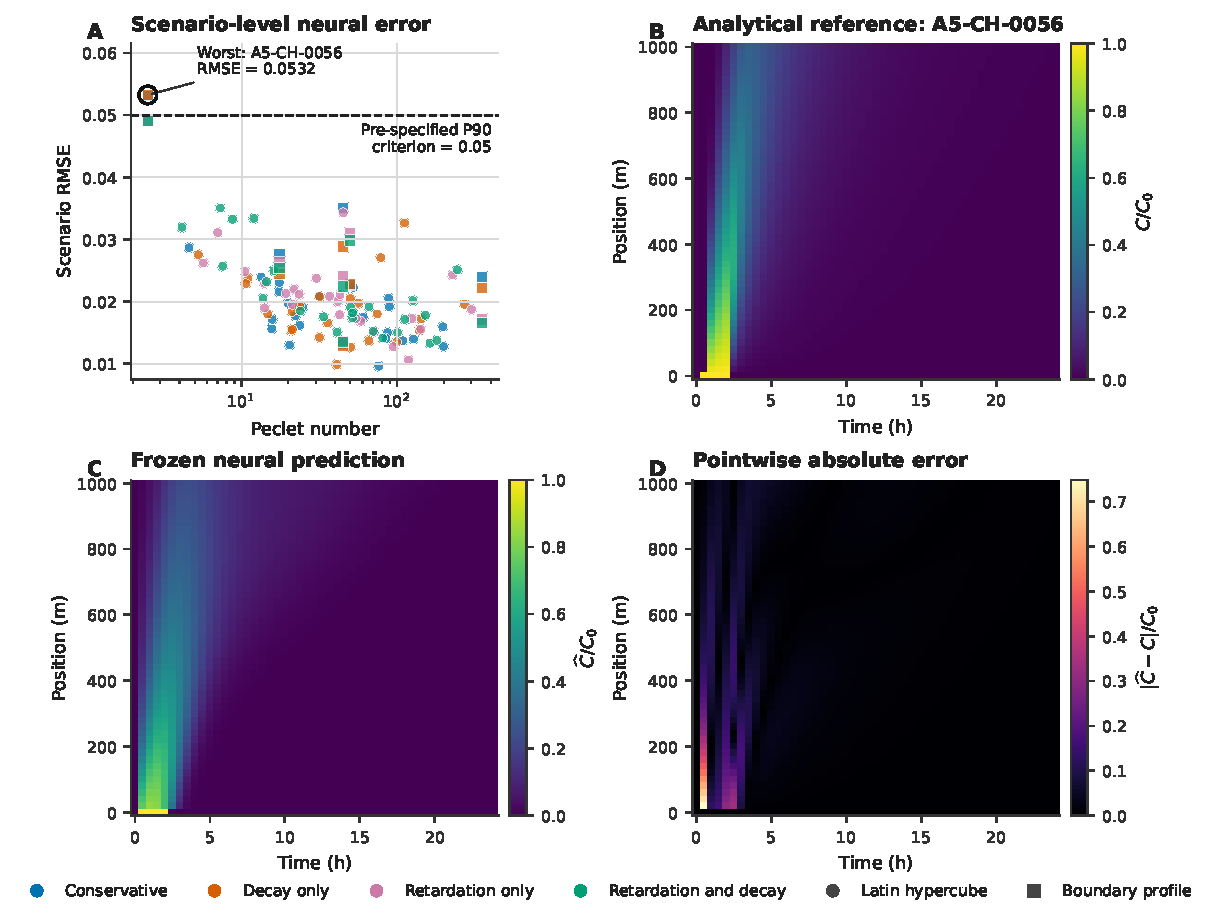
\includegraphics[width=0.92\textwidth]{figures/figure_02_neural_field_validation.pdf}
\caption{Heterogeneity of ADR1D-NN error. (A) Per-scenario RMSE versus Peclet
number; the criterion applies to the 90th percentile, not the individual
maximum. (B--D) Analytical reference, frozen prediction, and absolute error for
the scenario with the largest persisted RMSE, \code{A5-CH-0056}. Squares
identify boundary profiles and circles identify Latin hypercube points.}
\label{fig:nn}
\end{figure}

Case \code{A5-CH-0056} belongs to the decay-only regime, was a boundary profile,
and had $\mathrm{Pe}=2.5$. Its RMSE was 0.05323, $R^2=0.87276$, active RMSE was
0.03662, and maximum error was 0.74876. Figure~\ref{fig:nn} shows that the
difference is concentrated around the early evolution of the pulse and its
front rather than spread uniformly across the 24 h. The maximum pointwise
error in the entire challenge, 0.74945, occurred in another boundary profile
with Peclet 2.5, \code{A5-CH-0026}. The coexistence of a low global RMSE and
large maximum errors is explained in part by the large proportion of inactive
or near-zero cells.

The two maxima locate the mechanism. In \code{A5-CH-0056} and
\code{A5-CH-0026}, the source starts at $t=1800$ s, the first interior position
is $x=20$ m, and the reference remains zero at the exact activation time. The
network predicted 0.74876 and 0.74945, respectively. The point is not covered
by the hard constraints because it belongs to neither $t=0$ nor $x=0$. This is
an early interior arrival at a temporal discontinuity, not a small deviation
distributed throughout the field. Moreover, because the reference is less
than $10^{-4}$, these maxima belong by definition to the inactive region and
do not appear in the active maximum.

Boundary profiles had a pooled RMSE of 0.02995, compared with 0.02032 at Latin
hypercube points. The lowest Peclet quartile had a pooled RMSE of 0.03033, the
largest among quartiles. Active RMSE, however, was largest in the highest
Peclet quartile (0.05117), where the front occupies fewer points and active
errors have less weight in the global average. These observations support
examining both active regions and complete profiles. They also show that
``higher Peclet'' does not automatically imply a higher global RMSE: the upper
quartile has fewer active cells, so the total average is dominated by zeros
even though error within the front is larger.

No values fell outside $[0,1]$. The discrete PDE residual was
$1.961\times10^{-4}$ s$^{-1}$. It is reported as a diagnostic: it depends on
the discretization used to compute derivatives and does not constitute a test
of local conservation or exact satisfaction of the equation. Its value is not
compared directly with $\lambda$ because the residual combines temporal,
advective, dispersive, and reactive derivatives, and centered differences are
particularly sensitive to abrupt pulse changes.

\subsection{Numerical Reference and Refinement}

The local analytical implementation was first checked against 39,200 values
from the locked field; the maximum absolute difference was
$6.50\times10^{-12}$. The 16 selected cases were solved at three levels, for a
total of 48 runs. RMSE relative to the analytical solution decreased
monotonically in every case.

\begin{figure}[htbp]
\centering
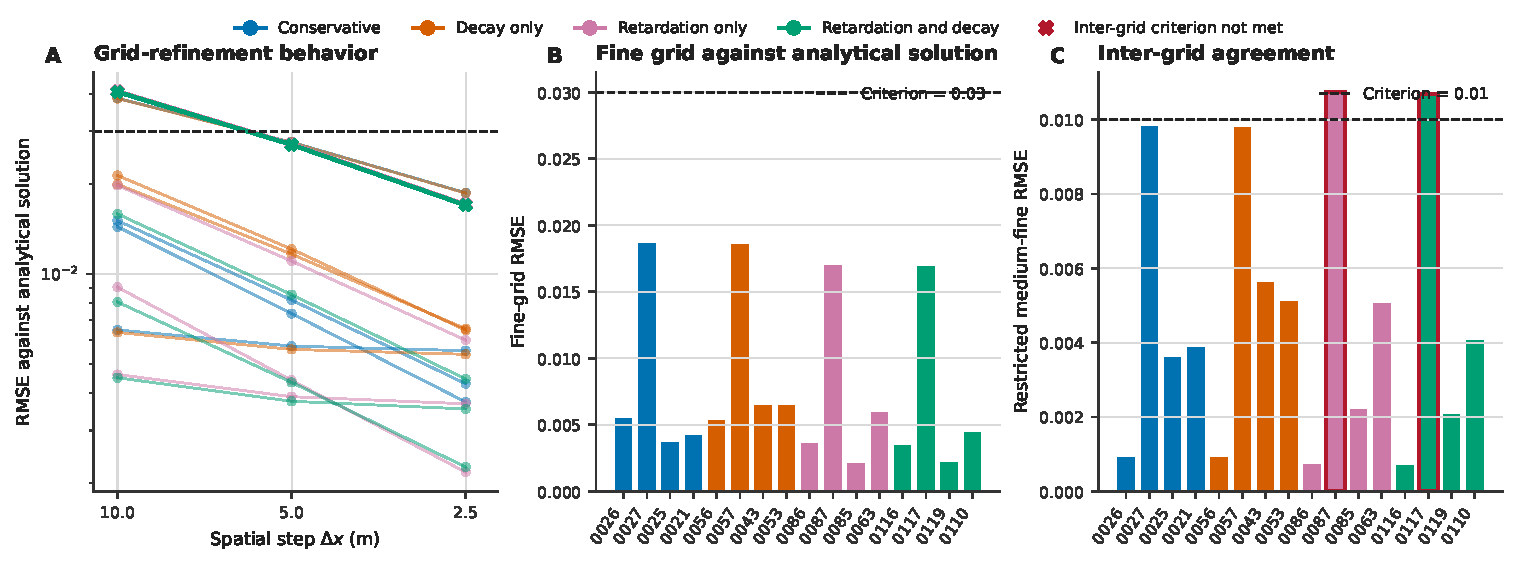
\includegraphics[width=\textwidth]{figures/figure_03_numerical_reference_convergence.pdf}
\caption{Traditional reference. (A) RMSE relative to the analytical solution
under space and time refinement. (B) Fine-mesh RMSE in the 16 cases. (C) RMSE
between medium and fine meshes restricted to common points. Red outlines mark
the two cases that exceeded the intermesh tolerance.}
\label{fig:numerical}
\end{figure}

\begin{table}[htbp]
\centering
\caption{Summary of the traditional numerical reference.}
\label{tab:numerical}
\small
\begin{tabularx}{\textwidth}{@{}YrrC@{}}
\toprule
Diagnostic & Observed & Criterion & Assessment \\
\midrule
Median fine-mesh RMSE & 0.00546 & $\leq0.03$ per case & \pass \\
Maximum fine-mesh RMSE & 0.01867 & $\leq0.03$ per case & \pass \\
Median medium--fine RMSE & 0.00399 & $\leq0.01$ per case & --- \\
Maximum medium--fine RMSE & 0.01074 & $\leq0.01$ per case & \mixed \\
Minimum normalized concentration & 0.0 & $\geq-10^{-10}$ & \pass \\
Maximum absolute balance residual & $4.45\times10^{-13}$ & Diagnostic & --- \\
\bottomrule
\end{tabularx}
\end{table}

Table~\ref{tab:numerical-cases} expands the aggregate result and permits review
of all 16 cases without relying on the figure. ``Medium--fine'' compares cell
averages on the same restricted mesh; the two bold values are the only ones
above 0.01.

\begin{table}[htbp]
\centering
\caption{Individual results from the traditional reference. Pe and Da are
computed from the true parameters.}
\label{tab:numerical-cases}
\scriptsize
\setlength{\tabcolsep}{3.5pt}
\begin{tabularx}{\textwidth}{@{}p{1.9cm}Yrrrr@{}}
\toprule
Case & Selection criterion & Pe & Da & Fine RMSE & Medium--fine RMSE \\
\midrule
\multicolumn{6}{@{}l}{\textbf{Conservative}} \\
\code{A5-CH-0026} & Minimum Pe & 2.50 & 0 & 0.00554 & 0.00094 \\
\code{A5-CH-0027} & Maximum Pe & 350.00 & 0 & 0.01867 & 0.00984 \\
\code{A5-CH-0025} & Maximum advective travel time & 50.00 & 0 & 0.00373 & 0.00363 \\
\code{A5-CH-0021} & Medoid & 31.48 & 0 & 0.00430 & 0.00389 \\
\addlinespace
\multicolumn{6}{@{}l}{\textbf{Decay only}} \\
\code{A5-CH-0056} & Minimum Pe & 2.50 & 0.02828 & 0.00539 & 0.00094 \\
\code{A5-CH-0057} & Maximum Pe & 350.00 & 0.00404 & 0.01863 & 0.00982 \\
\code{A5-CH-0043} & Maximum Da & 74.42 & 0.13230 & 0.00649 & 0.00565 \\
\code{A5-CH-0053} & Medoid & 50.33 & 0.00441 & 0.00655 & 0.00514 \\
\addlinespace
\multicolumn{6}{@{}l}{\textbf{Retardation and decay}} \\
\code{A5-CH-0116} & Minimum Pe & 2.50 & 0.05798 & 0.00354 & 0.00073 \\
\code{A5-CH-0117} & Maximum Pe & 350.00 & 0.00828 & 0.01697 & \textbf{0.01069} \\
\code{A5-CH-0119} & Maximum Da & 44.72 & 0.30000 & 0.00226 & 0.00208 \\
\code{A5-CH-0110} & Medoid & 51.73 & 0.01751 & 0.00445 & 0.00408 \\
\addlinespace
\multicolumn{6}{@{}l}{\textbf{Retardation only}} \\
\code{A5-CH-0086} & Minimum Pe & 2.50 & 0 & 0.00368 & 0.00073 \\
\code{A5-CH-0087} & Maximum Pe & 350.00 & 0 & 0.01704 & \textbf{0.01074} \\
\code{A5-CH-0085} & Maximum advective travel time & 50.00 & 0 & 0.00218 & 0.00223 \\
\code{A5-CH-0063} & Medoid & 58.58 & 0 & 0.00601 & 0.00509 \\
\bottomrule
\end{tabularx}
\end{table}

Fourteen scenarios met every criterion. \code{A5-CH-0117} (retardation with
decay) and \code{A5-CH-0087} (retardation only), both selected for maximum
Peclet and both with $\mathrm{Pe}=350$, produced medium--fine RMSE values of
0.01069 and 0.01074. The exceedances above 0.01 were small but were retained
without relaxing the threshold. Both cases did meet the fine-mesh tolerance
relative to the analytical solution, with RMSE values of 0.01697 and 0.01704.

The medium--fine exceedances were 6.9\,\% and 7.4\,\% relative to the tolerance,
not orders of magnitude. Their coincidence at $\mathrm{Pe}=350$ nevertheless
has a concrete numerical explanation. Cell Peclet is
$P_h=\mathrm{Pe}\,\Delta x/L$: it is 1.75 on the medium mesh and 0.875 on the
fine mesh. Both solutions remain stable and nonnegative because of exponential
fitting, but they represent a narrow front at different resolutions. The
intermesh criterion detects that displacement even though both solutions
maintain an RMSE below 0.03 relative to the analytical solution.

The largest fine-mesh RMSE, 0.01867, corresponded to the conservative case
\code{A5-CH-0027}, also with $\mathrm{Pe}=350$. This pattern is consistent with
the greater difficulty of resolving advection-dominated fronts at fixed
resolution. Median observed order was 0.681 from coarse to medium and 0.751
from medium to fine. These values describe the joint campaign in $\Delta x$
and $\Delta t$; they are not a formal asymptotic estimate of scheme order.

All concentrations were nonnegative, and the maximum absolute residual of the
discrete balance was $4.45\times10^{-13}$; the maximum relative residual was
$2.72\times10^{-9}$. The evidence supports the consistency of the reference in
the examined cases, but the two intermesh failures justify the aggregate
result of \emph{mixed evidence} and support further refinement when Peclet
approaches the upper end of the domain.

\subsection{Computational Cost}

Figure~\ref{fig:cost} and Table~\ref{tab:cost} present the medians of seven
repetitions. Interquartile ranges were narrow relative to the medians, and each
workload produced an identical output in the two warm-ups, the seven measured
repetitions, and the separate memory probe.

\begin{figure}[htbp]
\centering
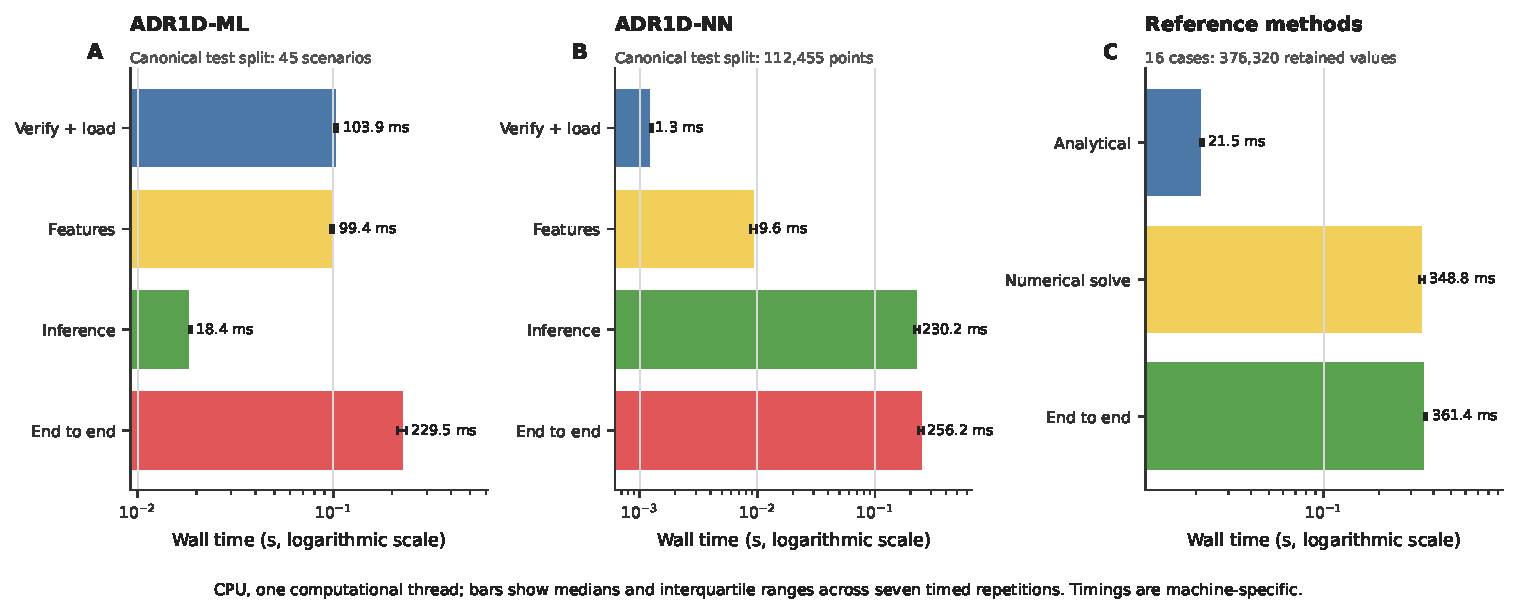
\includegraphics[width=\textwidth]{figures/figure_04_computational_cost.pdf}
\caption{Computational cost by component. Bars indicate the median and
interquartile range. Each panel has a different workload and should not be used
to compute a direct speed-up between models or methods.}
\label{fig:cost}
\end{figure}

\begin{table}[htbp]
\centering
\caption{Wall-clock times on a single CPU thread. IQR: interquartile range.}
\label{tab:cost}
\small
\begin{tabularx}{\textwidth}{@{}Yrrr@{}}
\toprule
Workload & Median (ms) & IQR (ms) & Median throughput \\
\midrule
ADR1D-ML: verify and load bundle & 103.87 & 2.90 & 9.63 loads s$^{-1}$ \\
ADR1D-ML: construct 45 rows & 99.41 & 3.02 & 452.7 scenarios s$^{-1}$ \\
ADR1D-ML: infer 45 scenarios & 18.44 & 0.42 & 2441.0 scenarios s$^{-1}$ \\
ADR1D-ML: end to end & 229.54 & 23.17 & 196.0 scenarios s$^{-1}$ \\
\addlinespace
ADR1D-NN: verify and load network & 1.25 & 0.04 & 799.5 loads s$^{-1}$ \\
ADR1D-NN: construct 112,455 rows & 9.55 & 1.11 & $1.177\times10^7$ points s$^{-1}$ \\
ADR1D-NN: infer 112,455 points & 230.24 & 23.24 & $4.884\times10^5$ points s$^{-1}$ \\
ADR1D-NN: end to end & 256.23 & 20.80 & $4.389\times10^5$ points s$^{-1}$ \\
\addlinespace
Analytical reference: 376,320 values & 21.50 & 0.75 & $1.750\times10^7$ values s$^{-1}$ \\
Traditional solution: 376,320 values & 348.84 & 20.20 & $1.079\times10^6$ values s$^{-1}$ \\
Numerical reference, end to end & 361.36 & 9.27 & $1.041\times10^6$ pairs s$^{-1}$ \\
\bottomrule
\end{tabularx}
\end{table}

Pure ADR1D-ML inference occupied a smaller fraction of total time; feature
construction and verification/loading contributed more. The opposite occurred
for ADR1D-NN: for 112,455 points, inference dominated the time and input
construction was brief. In the traditional reference, the numerical solution
dominated analytical evaluation.

Each row represents a complete batch, not the fixed cost of an isolated
prediction. Throughput in scenarios or points per second is obtained by
dividing batch cardinality by median time and may change with a different batch
size. In a service that keeps the model in memory, loading cost would be
amortized; in a command-line execution started for every query, it would be
paid again. This study reports both components but does not simulate a
persistent service.

These figures describe an Apple arm64 computer with macOS 26.5.2, 10 logical
CPUs, 24 GiB of memory, and CPython 3.12.2. The environment used NumPy 2.0.2,
pandas 2.2.3, SciPy 1.15.2, scikit-learn 1.7.0, joblib 1.4.2, and PyTorch 2.7.1.
The workloads are not equivalent: ADR1D-ML solves one inverse problem per
scenario, ADR1D-NN evaluates a pointwise surrogate, and the numerical reference
retains values from 16 cases on a different mesh. A speed-up factor is
therefore not computed.

The analytical solution was the fastest measured field operation. This
matters when interpreting the value of the surrogate: in the homogeneous ADR1D
problem, where a closed-form expression exists, the network offers no
demonstrated computational advantage over that expression. Its value for
integration must be evaluated in problems where the closed form is unavailable
or where it forms part of a broader workflow. The current campaign does not yet
measure that setting.

Peak memory traced from Python was approximately 27.6 MiB for ADR1D-ML loading
and the full workflow, 25.9 MiB for the complete ADR1D-NN workflow, and 11.5 MiB
for the complete numerical reference. These quantities exclude memory that
native libraries do not expose to \code{tracemalloc}.

\section{Discussion}

\subsection{What the Evaluation Demonstrates}

The main strength of the evidence is not a single $R^2$ value but the sequence
of controls: frozen models, a prior protocol, a collision-free challenge, one
persisted inference, an audit from flat outputs, per-scenario comparison, and
an independent traditional reference. Within that framework, ADR1D-ML retains
the ability to recover effective parameters, and ADR1D-NN reproduces fields
with low aggregate error.

For ADR1D-ML, velocity is the most stable and accurate output. Dispersion and
decay exhibit greater relative variation, consistent with the difficulty of
separating broadening, attenuation, and censoring from six noisy curves. The
resolvability classifier discriminates well, but its precision of 0.5588
precludes treating a positive class as confirmation of decay. Its most
reasonable use is to flag scenarios that require further estimation or
additional information.

For ADR1D-NN, the absence of nonphysical values and exact satisfaction of
imposed conditions are useful properties for integration into a numerical
workflow. Even so, the hard constraints cover only specific parts of the
problem. The maximum pointwise error and boundary profiles show that a network
can satisfy its contract and retain a favorable global RMSE while locally
displacing a front. Validation intended for maxima, arrival times, or
concentration thresholds must retain local diagnostics.

The traditional campaign supports the analytical reference in the 16 cases
and confirms that error decreases under refinement. The two intermesh
exceedances occur at maximum Peclet. They do not invalidate the other
comparisons, but they identify a specific condition under which medium
resolution cannot be treated as equivalent to fine resolution under the
adopted tolerance.

\subsection{Joint Interpretation of the Models}

Although ADR1D-ML and ADR1D-NN may occupy consecutive stages of a workflow,
this campaign validated them separately. ADR1D-ML received sensor data and was
compared with true parameters. ADR1D-NN received the true challenge parameters
directly, not the estimates from ADR1D-ML. The network RMSE therefore
quantifies its surrogate error when its physical inputs are known; it does not
include error from a preceding inverse problem.

This distinction has consequences. If a dispersion estimate with 25\,\% error
is supplied to the network, the resulting field may differ from the solution
computed with true dispersion even if ADR1D-NN approximates the supplied input
perfectly. Likewise, a false positive in resolvability may introduce a positive
$\lambda$ in a case whose attenuation cannot be separated from noise. Errors
from the two stages need not add linearly and may alter arrival times,
amplitudes, and areas in different ways.

The current evidence consequently permits the interfaces to be integrated in
controlled experiments, but does not permit the individual metrics of either
model to be assigned to the chained workflow. An end-to-end validation would
need to take the five sensor realizations, propagate the distribution of
parameters estimated by ADR1D-ML into ADR1D-NN, and compare the resulting
fields with the reference without replacing inputs by their true values.

\subsection{What the Evaluation Does Not Demonstrate}

The new scenarios belong to the same equation, geometry, and source family as
the development benchmark. They are an independent sample within the domain,
not a test of different physics. The validation also provides no field data in
which hydraulic velocity, dispersion, porosity, and boundary conditions are
observed simultaneously. Available WQP records provide context for
concentrations, units, censoring, and provenance, but cannot by themselves
reconstruct an identifiable case of Equation~\eqref{eq:adr}.

Bootstrap intervals quantify variation among scenarios in the design rather
than predictive uncertainty for an individual case. ADR1D-NN is deterministic,
and no ensembles, probabilistic calibration, or propagation of parameter
uncertainty were evaluated. Spatial, temporal, and parametric extrapolation
were likewise not tested.

The timing comparison does not isolate every implementation decision or
represent different hardware. Loading a tree bundle and loading a neural
checkpoint, in particular, do not have the same contract. Throughputs per
second help size this execution but should not be generalized without repeating
the benchmark in the target environment.

Table~\ref{tab:claim-boundaries} summarizes the boundaries of interpretation.

\begin{table}[H]
\centering
\caption{Claims supported and not supported by the campaign.}
\label{tab:claim-boundaries}
\small
\begin{tabularx}{\textwidth}{@{}Yp{2.3cm}Y@{}}
\toprule
Question & Answer & Reason \\
\midrule
Are the canonical evaluations reproduced? & Yes & The reconstructed reports
were identical byte for byte. \\
Do the models work separately on new cases within ADR1D? & Yes, with limits &
They met aggregate criteria but retained false positives and large local
errors. \\
Is the ADR1D-ML $\rightarrow$ ADR1D-NN chain validated? & No & The network
received true rather than inferred parameters. \\
Is use with field data validated? & No & Hydraulic parameters, boundary
conditions, and an identifiable observational reference are missing. \\
Has extrapolation been demonstrated? & No & All cases belong to the ADR1D
ranges, geometry, and equation. \\
Is there a universal speed-up? & No & Workloads, cardinalities, and computers
are not equivalent; the analytical solution was also faster in this case. \\
Are the criteria equivalent to regulatory safety? & No & They are engineering
tolerances specified for the synthetic benchmark. \\
\bottomrule
\end{tabularx}
\end{table}

\subsection{Implications for Numerical Integration}

The results support conditional integration rather than automatic replacement
of the physical model. The following practices are recommended:

\begin{enumerate}
    \item \textbf{Verify identity.} Checking the model, protocol, and inference
    modules against their manifests before loading an artifact avoids
    evaluating a version other than the documented one.
    \item \textbf{Validate inputs.} Reject or flag positions, times,
    parameters, and pulses outside ADR1D ranges. A numerically valid output
    does not turn extrapolation into evidence.
    \item \textbf{Retain replicates.} In the inverse problem, keep all five
    predictions and the resolvability probability, not only their means and
    classes, to represent sensitivity to noise.
    \item \textbf{Propagate parameters.} If ADR1D-ML feeds ADR1D-NN, evaluate
    several plausible parameter sets instead of treating a point estimate as
    exact truth.
    \item \textbf{Inspect the local field.} Accompany global RMSE with
    active-region error, arrival diagnostics, profiles near the source, and
    maxima. The two errors near 0.75 show why this step is needed.
    \item \textbf{Maintain sentinel cases.} Solve boundary combinations and
    high-Peclet cases with an analytical or numerical reference for every
    version of the integrated workflow.
    \item \textbf{Record cost by component.} Separate loading,
    transformation, and inference on the target hardware before choosing a
    deployment strategy.
    \item \textbf{Revalidate when physics changes.} Heterogeneity, different
    boundaries, multidimensional geometry, or site data constitute a new
    problem and require a new protocol and new evidence.
\end{enumerate}

In repeated simulations, ADR1D-NN may be useful as a field approximator and
ADR1D-ML as a preliminary inverse stage. Neither replaces the assessment of
identifiability, uncertainty propagation, or physical balance required by the
final application.

\section{Threats to Validity and Limitations}

\begin{itemize}
    \item \textbf{External validity.} The study is synthetic,
    one-dimensional, and homogeneous. It does not cover spatial heterogeneity,
    multidimensional transport, nonlinear reactions, or complete field data.
    \item \textbf{Physical independence.} The challenge uses a reconstructed
    implementation of the same analytical solution and the same physical
    ranges. Independence comes from the samples, locking, and audit rather than
    from a different transport theory.
    \item \textbf{Dependence between benchmark and models.} Both development
    and challenge labels come from ADR1D. The absence of collisions prevents
    repeated scenarios but does not remove shared assumptions about
    homogeneity, linearity, a rectangular pulse, and constant parameters.
    \item \textbf{Traditional reference.} Sixteen cases and three meshes were
    evaluated. This selection covers extremes and medoids but does not
    constitute an exhaustive convergence study.
    \item \textbf{Temporal resolution.} Arrival diagnostics use 1800 s steps
    in the challenge field; errors equal to that value are quantized by the
    evaluation table.
    \item \textbf{Noise.} The sensor model represents one combination of
    Gaussian error, an absolute floor, censoring, and substitution. It does not
    cover drift, temporal dependence, calibration bias, or sensor failures.
    \item \textbf{Conditional decay.} The $\lambda$ regression is summarized
    from 23 resolvable scenarios. Its intervals are wider than those for
    velocity and must be retained when accuracy is communicated.
    \item \textbf{Definition of resolvability.} The threshold
    $1-\exp(-\mathrm{Da})\geq0.03$ relates ideal attenuation to relative noise,
    but does not incorporate the absolute floor, censoring, or every
    correlation among parameters. It is an operational benchmark definition,
    not a universal limit of experimental detectability.
    \item \textbf{Unevaluated coupling.} ADR1D-NN received true parameters.
    The study does not quantify how ADR1D-ML errors and decisions propagate to
    the field.
    \item \textbf{Discontinuities.} The rectangular source changes
    instantaneously. The largest neural errors occur precisely near source
    activation and the first interior cell; other source forms may alter the
    error distribution.
    \item \textbf{Memory and time.} The benchmark was run on one computer. The
    Python memory probe may omit native allocations and is not equivalent to
    maximum resident memory.
    \item \textbf{Criteria.} The tolerances were specified before the
    challenge, but they are engineering criteria for this study rather than
    water-quality standards or guarantees for public decisions.
\end{itemize}

\section{Reproducibility and Traceability}

All results were stored in open CSV or JSON formats. The machine-readable
protocol is located at \path{configs/validation_protocol.json}. The primary
evidence is under \path{results/}, and generators and validators are under
\path{src/}. Only \path{src/evaluate_locked_challenge.py} executed new
inference on the challenge, once per model. Subsequent figure generation read
persisted results exclusively and recorded
\code{model\_loading\_or\_inference = false}.

Reproducibility was organized into three scopes. \emph{Integrity verification}
confirms that every expected file exists and corresponds to its
machine-readable record. The \emph{results audit} recalculates metrics and
intervals from persisted predictions without querying the models. A
\emph{complete reconstruction} regenerates cases or runs models and must be
performed in a temporary directory so that a replica is not confused with the
historical evidence. The final manifest uses the first two scopes and does not
increment the challenge-inference counter.

Paths stored in the manifests are relative to the validation directory, so the
collection can be moved to another computer without rewriting absolute paths.
Each JSON records versions, seeds, counts, and integrity information for its
inputs. Cryptographic fingerprints used by validators remain in those files
and are not duplicated in the report.

\begin{table}[htbp]
\centering
\caption{Primary traceability records and documented content.}
\label{tab:traceability}
\small
\begin{tabularx}{\textwidth}{@{}Yl@{}}
\toprule
Artifact & Status or content \\
\midrule
\path{validation_protocol.json} & Locked protocol \\
\path{challenge_scenarios.csv} & 120 scenarios \\
\path{challenge_analytical_field.csv} & 299,880 values \\
\path{challenge_sensor_observations.csv} & 176,400 observations \\
\path{canonical_reproduction.json} & Complete reproduction \\
\path{challenge_result_validation.json} & Passed audit \\
\path{numerical_reference_cases.csv} & 48 runs \\
\path{numerical_reference_metrics.json} & Mixed evidence \\
\path{computational_cost.json} & 11 measured workloads \\
\path{figure_manifest.json} & Eight graphical files \\
\bottomrule
\end{tabularx}
\end{table}

The four graphics are stored in both PDF and PNG. Two independent temporary
renderings produced identical files in all eight formats. The manifest records
the inputs, generator, and each figure, as well as the criterion that selected
\code{A5-CH-0056} for field inspection.

The cost audit verified 14 artifacts before and after execution, with no
changes, and recorded zero challenge inferences and zero newly persisted
predictions. The cost report also reproduced the canonical results of both
models and the numerical-reference RMSE values within tolerances below
$10^{-12}$.

The report itself is also part of traceability. Its internal date and PDF
trailer identifier were fixed before compilation; two builds in separate
directories must produce the same binary file. This condition verifies that
the delivered document corresponds to the LaTeX source and registered figures,
not that the scientific results are correct merely because it compiles.

\section{Conclusions}

The validation supports seven bounded conclusions:

\begin{enumerate}
    \item ADR1D-ML reproduced its canonical results and met every challenge
    criterion. Velocity estimation was the strongest output; dispersion and
    decay retained greater relative uncertainty.
    \item The resolvability classification distinguished the classes well in
    aggregate but produced 15 false positives and a precision of 0.5588.
    Probability and use context must accompany any positive class.
    \item ADR1D-NN achieved good global fit, preserved the physical interval,
    and imposed the hard conditions exactly. Maximum errors near 0.75 and the
    worst RMSE of 0.05323 show that a global summary does not replace analysis
    of fronts and boundary profiles.
    \item The traditional solution agreed with the analytical solution and
    improved monotonically in all 16 cases. Two scenarios with Peclet 350 did
    not meet the medium--fine tolerance; by design, the aggregate numerical
    result is mixed evidence.
    \item The observed times show that both models can be evaluated in
    fractions of a second for the tested workloads. Differences in task, mesh,
    and cardinality prevent converting these measurements into a universal
    speed-up.
    \item The two models were validated separately. ADR1D-NN received true
    parameters, so its metrics do not describe a workflow fed by ADR1D-ML.
    Propagation of inverse error into the field remains to be evaluated
    specifically.
    \item The models are ready for integration into controlled numerical
    experiments within the ADR1D domain, with input verification, retention of
    replicates, and physical checks. The evidence does not authorize
    extrapolation, field validation, or regulatory use without an additional
    campaign.
\end{enumerate}

The immediate next step is to evaluate the complete chain within the same
domain: noisy sensors, inferred parameters, neural field, and final comparison
with the reference. Subsequent work can examine how the evidence changes when
heterogeneity, different boundary conditions, and sufficient observations to
identify the physical problem are introduced. Every extension should retain
the same order: a prior protocol, frozen artifacts, local metrics, and
publication of both favorable and unfavorable results.

\section*{Declarations}
\addcontentsline{toc}{section}{Declarations}

\textbf{Author contributions.} Gerardo Tinoco-Guerrero, Francisco J.
Domínguez-Mota, and J. Alberto Guzmán-Torres contributed equally to the design,
analysis, interpretation, and review of the work.

\textbf{Conflicts of interest.} The authors declare no conflicts of interest.

\textbf{Funding and institutional support.} This work received funding and
institutional support from the Secretariat of Science, Humanities, Technology
and Innovation (SECIHTI) of Mexico; the Coordination of Scientific Research at
the Universidad Michoacana de San Nicolás de Hidalgo (CIC-UMSNH); SIIIA MATH:
Soluciones en Ingeniería; the International Centre for Numerical Methods in
Engineering (CIMNE); and Aula CIMNE Morelia.

\textbf{Data and code availability.} The original ADR1D data are available at
\url{https://github.com/gstinoco/ADR1D}. The models are published at
\url{https://github.com/gstinoco/ADR1D-ML} and
\url{https://github.com/gstinoco/ADR1D-NN}. Evidence specific to this validation
is preserved with this report in readable and auditable CSV, JSON, PDF, and
Python files.

\clearpage
\begingroup
\footnotesize
\setlength{\parskip}{0pt}
\begin{thebibliography}{99}
\setlength{\itemsep}{2pt}
\setlength{\parsep}{0pt}

\bibitem{adr1d}
G. Tinoco-Guerrero, F. J. Domínguez-Mota, and J. A. Guzmán-Torres,
\emph{ADR1D: A Reproducible One-Dimensional Contaminant-Transport Benchmark},
version 1.0.0, Universidad Michoacana de San Nicolás de Hidalgo, 2026.
\url{https://github.com/gstinoco/ADR1D}.

\bibitem{adr1dml}
G. Tinoco-Guerrero, F. J. Domínguez-Mota, and J. A. Guzmán-Torres,
\emph{ADR1D-ML: Identifiable Parameter Inference for One-Dimensional Reactive
Transport}, version 1.0.0, Universidad Michoacana de San Nicolás de Hidalgo,
2026. \url{https://github.com/gstinoco/ADR1D-ML}.

\bibitem{adr1dnn}
G. Tinoco-Guerrero, F. J. Domínguez-Mota, and J. A. Guzmán-Torres,
\emph{ADR1D-NN: A Physics-Constrained Neural Surrogate for One-Dimensional
Reactive Transport}, version 1.0.0, Universidad Michoacana de San Nicolás de
Hidalgo, 2026. \url{https://github.com/gstinoco/ADR1D-NN}.

\bibitem{ogata1961}
A. Ogata and R. B. Banks, \emph{A Solution of the Differential Equation of
Longitudinal Dispersion in Porous Media}, U.S. Geological Survey Professional
Paper 411-A, 1961. \url{https://doi.org/10.3133/pp411A}.

\bibitem{chen2011}
J.-S. Chen and C.-W. Liu, ``Generalized analytical solution for
advection-dispersion equation in finite spatial domain with arbitrary
time-dependent inlet boundary condition,'' \emph{Hydrology and Earth System
Sciences}, vol. 15, pp. 2471--2479, 2011.
\url{https://doi.org/10.5194/hess-15-2471-2011}.

\bibitem{mckay1979}
M. D. McKay, R. J. Beckman, and W. J. Conover, ``A comparison of three methods for
selecting values of input variables in the analysis of output from a computer
code,'' \emph{Technometrics}, vol. 21, no. 2, pp. 239--245, 1979.
\url{https://doi.org/10.1080/00401706.1979.10489755}.

\bibitem{scharfetter1969}
D. L. Scharfetter and H. K. Gummel, ``Large-signal analysis of a silicon Read
diode oscillator,'' \emph{IEEE Transactions on Electron Devices}, vol. 16,
no. 1, pp. 64--77, 1969.
\url{https://doi.org/10.1109/T-ED.1969.16566}.

\bibitem{efron1993}
B. Efron and R. J. Tibshirani, \emph{An Introduction to the Bootstrap}.
New York: Chapman \& Hall/CRC, 1993.

\end{thebibliography}
\endgroup

\end{document}
